
\section{Software to be used in the pipeline}
A wide variety of software will be used across the MLOps pipeline, with an overall glossary of them documented in Table \ref{tab:softwareDescriptions}.
Descriptions on how they will specifically be used in each stage of the pipeline can be found in each stage's respective
section.

\begin{longtable}{ |p{0.2\textwidth}| p{0.8\textwidth}|}
    \hline
    \cellcolor{blue!25}Software/Library & \cellcolor{blue!25}Overview\\
    \hline
    Conda 
    & A package and environment management system which allows 
    for software developers and data scientists to easily control the libraries used in their code \autocite{anaconda_about_nodate}. 
    Allows for the creation of \textbf{virtual environments}, which are contained structures where packages can be installed.
    The use of virtual environments allows for specific versions of packages to be kept, for instance with one environment 
    storing an older version of a library for compatibility purposes, with another storing a newer version to be used in a different project. 
    Were it not for these virtual environments, developers would constantly have to uninstall and reinstall specific package versions, wasting 
    considerable amounts of time. Conda also hosts its own repositories to obtain packages from, and a 
    major benefit of Conda occurs during the package installation process, which is that it will identify 
    dependencies and version clashes between packages and solve them automatically, once again saving 
    considerable amounts of time.
    
    In this project, Conda will be used as the environment and package manager to install and contain the 
    libraries used in the development process. To do so, the Miniconda distribution will be installed, as 
    this is a smaller distribution to save hard disk space and download time, but still contains the key 
    Conda backend, as seen in Figure \ref{fig:Miniconda}. \\
    \hline
    Apache Airflow &
    A platform used to orchestrate workflows and pipelines entirely in Python code \autocite{apache_use_nodate}.
    Airflow creates Directed Acyclic Graphs (DAGs), which map out the order and dependencies of each task in a 
    pipeline, and runs tasks in the order specified within the DAG, while also accounting for dependencies.
    Also provides many useful features such as task scheduling, which is especially useful for the automation 
    of an MLOps pipeline, as well as automatic failure handling, where actions can automatically be performed 
    on a task's failure, such as stopping the pipeline to prevent wasting computational resources. Airflow 
    also provides a convenient UI, accessible by using the command "airflow webserver", which will host a 
    web UI where tasks can be run, paused or stopped, as well as viewed in a tree view that maps the 
    sequence and dependencies of tasks. Airflow also provides "Operators", which handle running code such 
    as Python and Bash scripts.

    Airflow will be used within this project at all stages of the pipeline in order to manage the overall 
    execution and structure of tasks. Operators will be used for the execution of all Python or Bash 
    commands throughout the pipeline. By using Airflow in this way, the pipeline can become completely 
    automated with continuous integration and continuous deployment.
    \\
    \hline
    Docker &
    An open-source containerisation system used to enhance the portability of applications by distributing 
    them as self-contained, lightweight instances that come with everything they need to run immediately 
    without needing to worry about system incompatibility (\textcite{aws_what_nodate}, \textcite{docker_docker_2022})
    and minimise issues where software can run on one computer but not another. Docker could be described 
    as working similarly to a virtual machine, though it is considerably more lightweight as it is not 
    virtualising hardware.\\
    \hline
    MariaDB Columnstore &
    A columnar storage engine designed for the processing of petabytes of data with high performance 
    and real-time response regardless of dataset size \autocite{mariadb_mariadb_nodate}. While 
    primarily intended for OLAP databases, it also facilitates OLTP databases. A Docker container 
    for this software will be used in this pipeline.\\
    \hline 
    Redis &
    An in-memory data store used to cache data in a machine's RAM rather than its 
    persistent storage. The benefits of this are that said data can be loaded many times faster than if 
    it were loaded from a hard drive. This does therefore mean that Redis will not be used to store persistent data,
    and it will instead be used to transfer data between different tasks in an Airflow DAG, as Airflow tasks 
    are independent from each other. Redis will solve this by having relevant data loaded into memory before 
    the task ends, at which point it will be read by the following task. A Docker container for this 
    software will be used in this pipeline. Also includes a Python library of the same name that allows 
    for access to the Redis store from Python scripts.\\
    \hline
    Direct-Redis &
    A package that builds upon the functionality of the normal Redis Python package by performing 
    automatic serialization and deserialization of data whenever data is sent or retrieved from the 
    connected Redis store \autocite{direct-redis_direct-redis_nodate}.\\
    \hline
    Pandas &
    A library used widely in industry for data analytics. It is capable of importing data of various 
    types and storing them in a "DataFrame" object, which preprocessing operations can be performed on.
    It also allows the exporting of data in multiple formats \autocite{pandas_pandas_nodate}.\\
    \hline
    SQLAlchemy &
    A library that allows SQL engine connections to be made from within a Python file. In 
    doing so, data can be read from and stored into SQL databases \autocite{sqlalchemy_sqlalchemy_nodate}.\\
    \hline
    Scikit-learn & 
    A large open-source Python library containing many different functionalities for machine learning \autocite{scikit-learn_scikit-learn_nodate}, 
    such as encoders to convert strings to numerical equivalents, scalers to normalise and standardise 
    the data to reduce variance (described further in Section \ref{sec:Preprocessing}), as well as containing 
    methods to split data into training and testing sets, and fit, train and predict with various different 
    machine learning algorithms (described further in Section \ref{sec:Development}).\\
    \hline
    FastAPI &
    A high-performance framework for developing APIs in Python, proclaimed
    as "One of the fastest Python frameworks available" \autocite{fastapi_fastapi_nodate}.
    Facilitates an API for clients to access the backend ML model later in the pipeline. \\
    \hline
    Uvicorn &
    A low-level webserver implementation in Python with high performance \autocite{uvicorn_uvicorn_nodate}.\\
    \hline
    MLFlow &
    An open-source platform for the tracking and monitoring of machine learning models, 
    storing each iteration of the model so that they may be reproduced at a later point \autocite{mlflow_mlflow_nodate},
    which is especially useful while performing hyperparameter tuning on the model, which is where 
    small details of the model are changed such as the number of decision trees in a Random Forest.
    Also facilitates REST APIs, discussed in Section \ref{sec:Deployment}.\\
    % \hline
    % Apache Arrow \newline PyArrow &
    % Software with a Python library interface that allows for the serialization of objects \autocite{apache_streaming_nodate}. 
    % This is important in synergy with Redis and Pandas, as Redis is unable to directly store Pandas dataframes, 
    % so they must first be serialized, converting them to a bytes format that Redis can store in memory.\\
    \hline
    Pickle &
    A base package in Python that is used to serialize data \autocite{python_pickle_nodate}.
    In this specific case, Pickle will be used to serialize machine learning models and save them 
    to a file that can be loaded for later predictions.\\
    \hline
    Great Expectations &
    A Python library used for data validation, where "expectations" can be set for a dataset, such as 
    all data of a column being numeric, and they will be assessed \autocite{gx_gx_nodate}.\\
    \hline
\caption{Descriptions of software and libraries across the pipeline.}\label{tab:softwareDescriptions}
\end{longtable}

\begin{figure}[H]
    \centering
    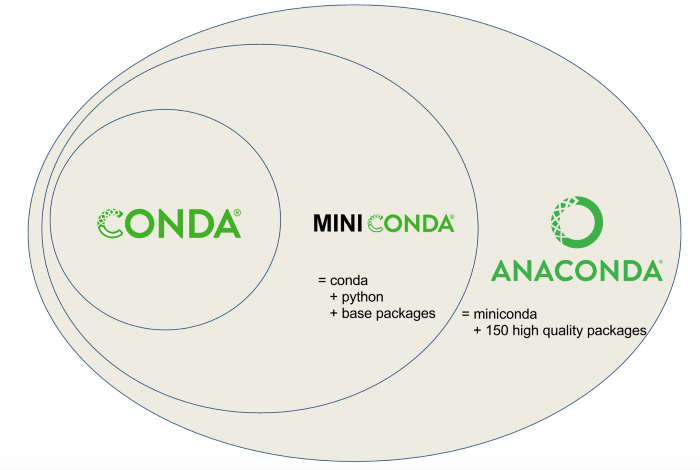
\includegraphics[width=.75\linewidth]{Draft Pipeline/miniconda.png}
    \caption{A comparison of the primary Conda distributions \autocite{towardsdatascience_getting_2021}}
    \label{fig:Miniconda}
\end{figure}

\pagebreak

\section{Data Ingestion}\label{sec:Ingestion}
% \subsubsection{Input: Raw Data from Original Source (Loan CSV from Kaggle)\\Output: Ingested Data (Data in MariaDB Columnstore)}
\subsection{Description}
The first step of any machine learning pipeline is data ingestion. This refers to the process of obtaining the input data from its original source
and transferring it to a relevant storage medium, such as a database or data warehouse, to be used in later stages. This stage 
is undertaken by data scientists. 
It is of vital importance that data is not lost or corrupted during ingestion, as this stage is the baseline for all future stages in the pipeline, and any issues
here will directly impact all future stages, as previously discussed. Furthermore, when ingesting data, it is important to understand what type of system this data 
will be used in, of which there are two options: Online Analytics Processing Systems (OLAP), and Online Transactional Processing Systems (OLTP), as well 
as how it will be loaded into the chosen system, either using an ELT (Extract, Load, Transform) or ETL (Extract, Transform, Load) methodology.

\subsubsection{OLAP and OLTP}

\begin{table}[H]
    \centering
        \begin{tabular}{ |p{0.4\textwidth}| p{0.425\textwidth}|}
            \hline
            \cellcolor{blue!25}OLAP & \cellcolor{blue!25}OLTP\\
            \hline
            Designed for complex queries and data analysis, primarily data reading.
            & Designed for lots of short, fast queries ("transactions") for both reading and writing.\\
            \hline
            Typically store massive amounts of data, sometimes petabytes.
            for extremely detailed analysis. 
            & Usually store less data for speed purposes.\\
            \hline
            Usually historical data, infrequently updated. 
            & Typically real-time data that is updated often.\\
            \hline 
            Uses database schemas such as star or snowflake schema to allow for queries using many joins. 
            & Uses normalised or denormalised models, such as One Big Table, minimising joins and maximising speed.\\
            \hline
            Slow response times, measured in minutes. 
            & Fast response times, measured in milliseconds.\\
            \hline
    \end{tabular}
    \caption{A comparison of OLAP and OLTP systems \autocite{aws_oltp_nodate}.}\label{tab:OLAP-OLTP}
\end{table}

As mentioned in Table \ref{tab:OLAP-OLTP}, OLAP systems are designed for complex and deep data analytics, which helps 
companies perform tasks such as analysing customer trends, while OLTP systems aim for maximum speed to complete quick transactions, 
which is necessary in situations like processing payments and orders.

\subsubsection{ELT and ETL}
ELT and ETL are both acronyms for the order of processes taken when ingesting data, with "Transform" either 
happening before or after the data is loaded into a storage medium like a data warehouse or data lake. 
The extract phase refers to the initial gathering of the data from its original source, such as Kaggle for 
the selected dataset in this report. The transform phase refers to early modifications made to the data, such 
as formatting or cleaning, and the load phase refers to the transportation of the data from its original storage
medium (a CSV on Kaggle's cloud servers in this case) to a more optimised and efficient data warehouse to be used 
in the execution of the pipeline.

Regardless of whether ETL or ELT is used, the data is still extracted, loaded and transformed. However,
the decision of which order to use can be determined from the data itself, with smaller datasets that may need 
complex transformation from their raw form being more suited to ETL, whereas large datasets with less 
transformation needed can be better with ELT \autocite{smallcombe_etl_nodate}.

\begin{table}[H]
    \centering
        \begin{tabular}{ |p{0.4\textwidth}| p{0.425\textwidth}|}
            \hline
            \cellcolor{blue!25}ELT & \cellcolor{blue!25}ETL\\
            \hline
            Data is transformed \textbf{after} being loaded into another storage medium.
            & Data is transformed \textbf{before} being loaded into another storage medium. \\
            \hline
            Useful if the data warehouse is a more modern system with good processing power.
            & Useful if the data warehouse has limited processing abilities of its own,
            typically seen in older or otherwise less powerful systems such as those on 
            virtual machines.\\
            \hline
            Lower latency in the ingestion phase because data is immediately loaded. 
            & Higher latency in the ingestion phase, because the data is being processed first, 
            adding an extra time overhead where the pipeline could be held up.\\
            \hline 
            Simpler to set up due to the immediate loading of the data.
            & Can be complex to set up and maintain, as the transformation would occur outside the warehouse.\\
            \hline
    \end{tabular}
    \caption{A comparison of ETL and ELT methodologies (\textcite{bartley_etl_2024}, \textcite{aws_etl_nodate}).}\label{tab:ELT-ETL}
\end{table}

It can be surmised from the analysis of each method in Table \ref{tab:ELT-ETL} that ETL is best applied 
to older systems with limited processing power, whereas ELT is better in more modern systems. 
It can additionally be argued that performing the ETL order of operations blurs the line between the ingestion and 
preprocessing stages, as the data is transformed before it is actually loaded into the system and
fully ingested, whereas ELT has a clear split between the ingestion and preprocessing of the data. 

\subsection{In this project}
The candidate dataset's raw CSV file, downloaded directly from Kaggle, will act as the input for this stage. It utilises the One Big Table schema, 
and it was previously established in Section \ref{sec:Dataset} that it contains no missing values. 
The size of the dataset is the largest of the three candidates but is still
small in comparison to those used in industry, being only 3.5MB in comparison to gigabytes and petabytes as previously 
mentioned in Table \ref{tab:OLAP-OLTP}. Because of this small size, processing operations performed on the dataset 
will be very fast, even with limited processing power, so the ETL methodology will be used to ingest the data 
into a MariaDB Columnstore OLTP database for quick and efficient loading and querying, where the end user will be 
able to quickly supply predictor variables and receive a fast response. To do so, 
some of the software originally mentioned in Table \ref{tab:softwareDescriptions} will be used, seen in Table \ref{tab:IngestionSoftware}.




\begin{longtable}{ |p{0.2\textwidth}| p{0.5\textwidth}|}
    \hline
    \cellcolor{blue!25}Software/Library & \cellcolor{blue!25}Usage for ingestion\\
    \hline
    Docker &
    In this stage, Docker will be used to host a container of MariaDB Columnstore.\\
    \hline
    MariaDB Columnstore &
    In this stage, the Columnstore will be hosted on a Docker container at port 3306 \autocite{docker_hub_mariadbcolumnstore_nodate}, 
    and will be used as the OLTP storage medium of the ingested data.\\
    \hline 
    Pandas &
    In the ingestion phase, it will be used to import the dataset's CSV file, and export it as SQL to 
    the MariaDB Columnstore through the use of SQLAlchemy.\\
    \hline
    SQLAlchemy &
    Alongside Pandas, SQLAlchemy will export the DataFrame to the MariaDB Columnstore instance.\\
    \hline 
    Great Expectations & When ingesting the data, Great Expectations will be used to validate that it is as expected.\\
    \hline
\caption{Software to be used in ingestion.}\label{tab:IngestionSoftware}
\end{longtable}

\begin{figure}[H]
    \centering
    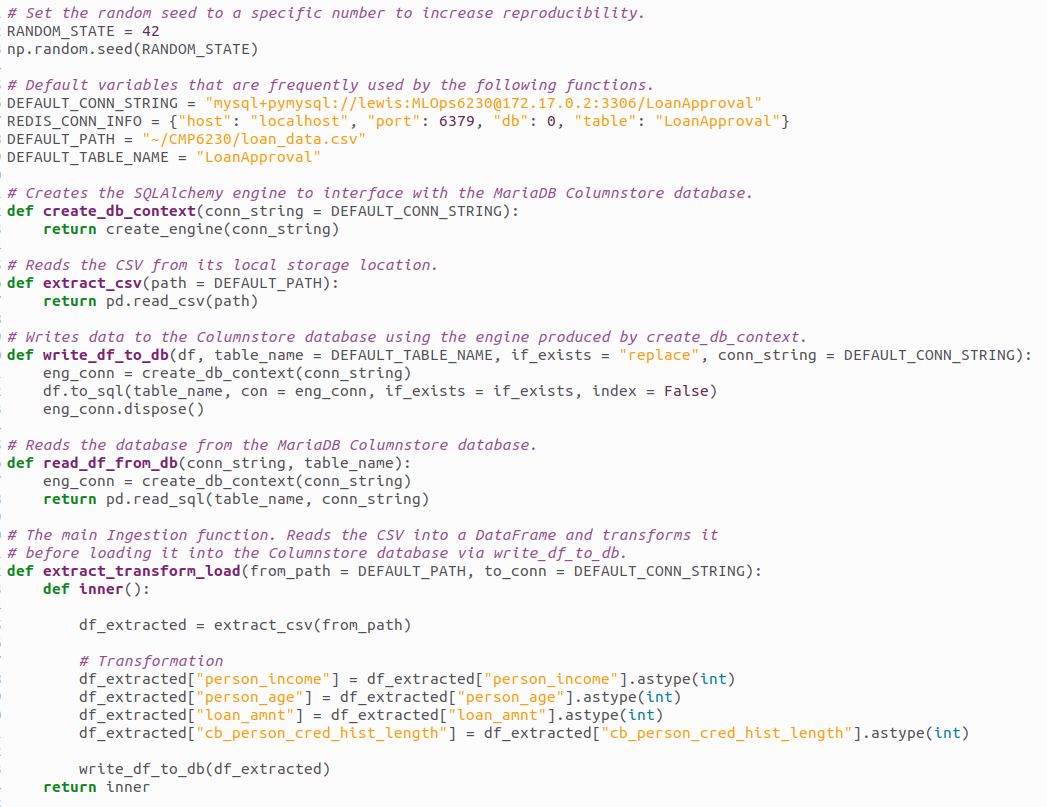
\includegraphics[width=.9\linewidth]{Draft Pipeline/diagrams/Ingestion.png}
    \caption{A diagram of the planned ingestion process.}
    \label{fig:IngestionDiagram}
\end{figure}

\pagebreak % separating Fig 2.3 from preprocessing section.

\section{Data Preprocessing}\label{sec:Preprocessing}
\subsection{Description}
After the data has been ingested, the preprocessing stage begins, and is often also conducted by 
Data Scientists. This stage encompasses the
cleaning, integration and transformation of the data in order to optimise the dataset for model development.

Cleaning refers to the identification of missing, inaccurate or malformed data within the dataset,
as well as its removal or imputation where possible.

Integration is often seen in datasets with multiple tables or that have been retrieved from multiple sources,
and refers to the combination of the retrieved data into a single flat file. 

Transformation, also known as feature engineering, is a considerable aspect of data preprocessing
which refers to the manipulation and formatting of the data, such as changing the formats of columns 
from numeric dates to proper date data types, as well as the handling of categorical data, such as genders, 
which may originally be strings. Strings cannot be interpreted by machine learning models, and therefore they 
are encoded into numbers using techniques such as label encoding, which converts the unique values in a column
to a numerical representation, such as male being 0 and female being 1. Data is also normalised and standardised 
in this stage, meaning that numerical data is reduced to being between 0 and 1 to adjust the overall scale of the 
data. This is especially useful with algorithms such as K-Nearest Neighbours, where large differences in distance 
between data can mislead the classification algorithm \autocite{ibm_what_2021}.

Once these tasks have all been completed, the dataset will be ready to be used for model development.

\subsection{In this project}
The preprocessing in this project will take the ingested data as input, from which point it will be transformed,
with columns such as "person\_gender" encoded to categorically labelled numerical equivalents. To do so, some of the software
and libraries originally mentioned in Table \ref{tab:softwareDescriptions} will be used, shown below in Table \ref{tab:PreprocessingSoftware}.
After this, the processed dataset will be output to Redis, to be used as the input for the model development stage.


\begin{longtable}{ |p{0.2\textwidth}| p{0.5\textwidth}|}
    \hline
    \cellcolor{blue!25}Software/Library & \cellcolor{blue!25}Usage for preprocessing\\
    \hline
    Pandas & 
    Will be used alongside SQLAlchemy to load the dataset from the MariaDB Columnstore instance hosted on Docker, 
    as well as for the actual transformation of the data using the methods provided by Pandas dataframes.\\
    \hline
    SQLAlchemy & 
    Will be used alongside Pandas to query and receive data from the MariaDB Columnstore instance.\\
    \hline
    Scikit-learn & 
    Will be used to normalise and standardise the data, as well as encode any string data into numerical 
    equivalents.\\
    \hline
    Docker &
    Will host the MariaDB Columnstore container. Additionally for this section, it will also host a 
    container for Redis to store the processed dataset.\\
    \hline
    Redis &
    Will store the processed dataframe in memory. Cannot directly store the dataframe as mentioned in 
    Table \ref{tab:softwareDescriptions}, so Direct-Redis acts as a wrapper that will also serialize it.\\
    \hline
    Direct-Redis & 
    Will serialize the processed dataframe before passing it to Redis.\\
    \hline
\caption{Descriptions of software to be used for preprocessing.}\label{tab:PreprocessingSoftware}
\end{longtable}

\begin{figure}[H]
    \centering
    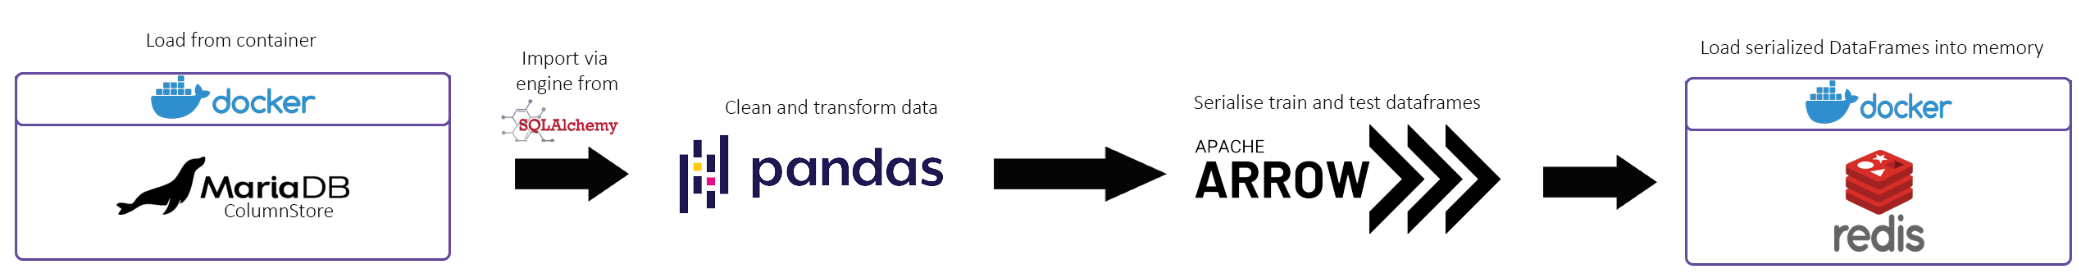
\includegraphics[width=.9\linewidth]{Draft Pipeline/diagrams/Preprocessing.png}
    \caption{A diagram of the planned preprocessing stage.}
    \label{fig:PreprocessingDiagram}
\end{figure}


\pagebreak

\subsection{Exploratory Data Analysis \& Research Questions}\label{subsec:EDA}
To build a machine learning model for a dataset, it greatly helps to understand the data itself. To do so, 
there are some key questions that can be answered through detailed data analysis, detailed below in Table \ref{tab:Questions}.

\begin{longtable}{ | p{0.05\textwidth} | p{0.85\textwidth} | }
    \hline
    \cellcolor{blue!25} ID & \cellcolor{blue!25} Question \\
    \hline
    1 & What is the age distribution of loan applicants? \\
    \hline
    2 & What is the most common intent for a loan? \\
    \hline
    3 & Does age influence loan approval rates? \\
    \hline 
    4 & Are more loans granted to men or women? \\
    \hline 
    5 & How does credit score influence the interest rate on a loan? \\
    \hline 
    6 & What is the most significant factor in the loan approval decision? \\
    \hline
    \caption{The questions that this EDA process aims to answer.}\label{tab:Questions}
\end{longtable}

\para These questions will be answered thoroughly throughout this section and in 
Table \ref{tab:Answers}.


\subsubsection{Distributions and outliers}
Understanding the data also means knowing how the data is typically distributed, and what constitutes an outlier. This can be 
done through visualisations such as box plots for numerical data and bar charts for categorical data.

\begin{figure}[H]
    \centering
    \begin{subfigure}[b]{0.3\textwidth}
        \centering
        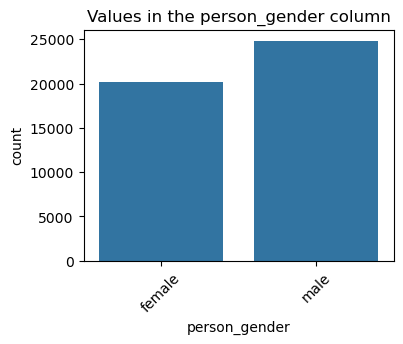
\includegraphics[width=\textwidth]{Plots/Gender.png}
        \caption{Genders}
        \label{fig:Bar1}
    \end{subfigure}
    \hfill
    \begin{subfigure}[b]{0.3\textwidth}
        \centering
        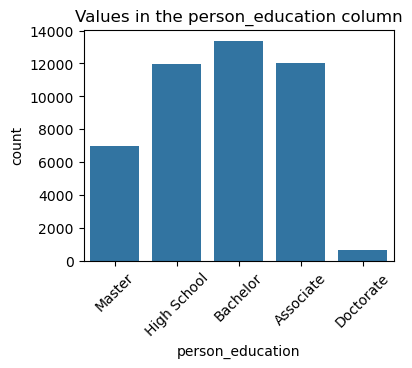
\includegraphics[width=\textwidth]{Plots/Education.png}
        \caption{Education levels}
        \label{fig:Bar2}
    \end{subfigure}
    \hfill
    \begin{subfigure}[b]{0.3\textwidth}
        \centering
        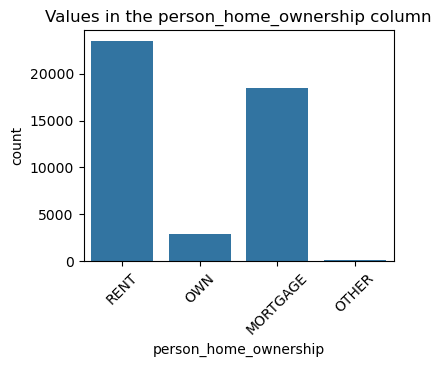
\includegraphics[width=\textwidth]{Plots/HomeOwnership.png}
        \caption{Home ownership}
        \label{fig:Bar3}
    \end{subfigure}
    
    \vspace{1em}
    
    \begin{subfigure}[b]{0.3\textwidth}
        \centering
        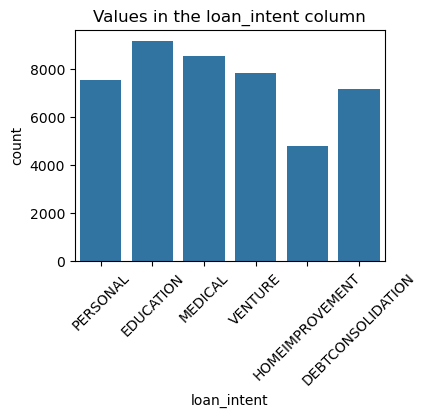
\includegraphics[width=\textwidth]{Plots/LoanIntent.png}
        \caption{Loan intents}
        \label{fig:Bar4}
    \end{subfigure}
    \hfill
    \begin{subfigure}[b]{0.3\textwidth}
        \centering
        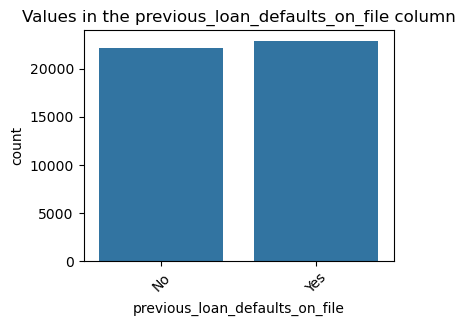
\includegraphics[width=\textwidth]{Plots/DefaultsOnFile.png}
        \caption{Previously defaulted}
        \label{fig:Bar5}
    \end{subfigure}
    \hfill
    \begin{subfigure}[b]{0.3\textwidth}
        \centering
        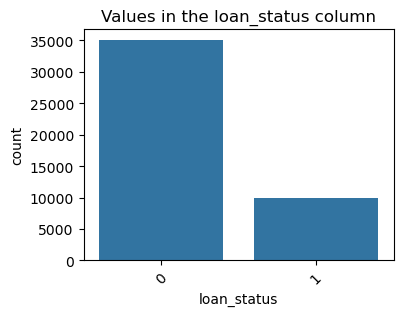
\includegraphics[width=\textwidth]{Plots/LoanStatus.png}
        \caption{Loan status}
        \label{fig:Bar6}
    \end{subfigure}
    \caption{Bar charts of the six categorical rows.}
    \label{fig:BarCharts}
\end{figure}

\para A notable observation is that the dataset is imbalanced, containing fewer records of granted 
loans than denied loans. Additionally, the most common loan intent as inquired by Question 2 is for 
educational purposes, such as university student loans.

\begin{figure}[H]
    \centering
    \begin{subfigure}[b]{0.22\textwidth}
        \centering
        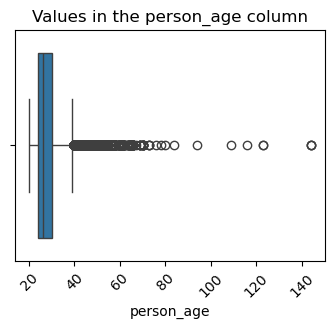
\includegraphics[width=\textwidth]{Plots/Age.png}
        \caption{Age}
        \label{fig:Boxplot1}
    \end{subfigure}
    \hfill
    \begin{subfigure}[b]{0.22\textwidth}
        \centering
        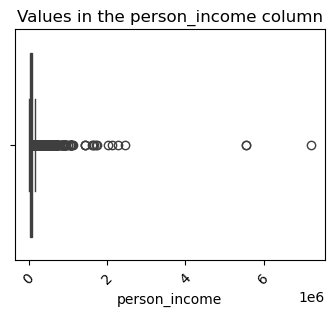
\includegraphics[width=\textwidth]{Plots/Income.png}
        \caption{Yearly income}
        \label{fig:Boxplot2}
    \end{subfigure}
    \hfill
    \begin{subfigure}[b]{0.22\textwidth}
        \centering
        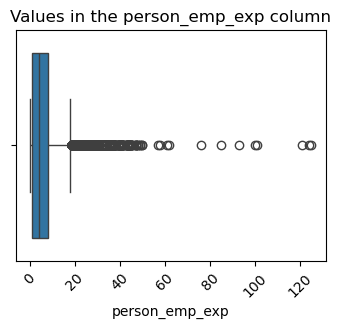
\includegraphics[width=\textwidth]{Plots/Employment.png}
        \caption{Previous jobs}
        \label{fig:Boxplot3}
    \end{subfigure}
    \hfill
    \begin{subfigure}[b]{0.22\textwidth}
        \centering
        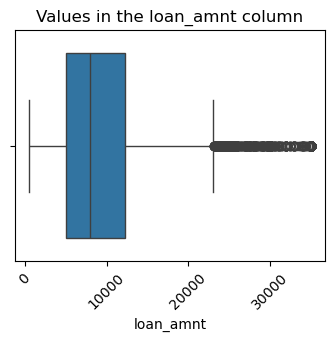
\includegraphics[width=\textwidth]{Plots/LoanAmount.png}
        \caption{Loan amount}
        \label{fig:Boxplot4}
    \end{subfigure}
    
    \vspace{1em}
    
    \begin{subfigure}[b]{0.22\textwidth}
        \centering
        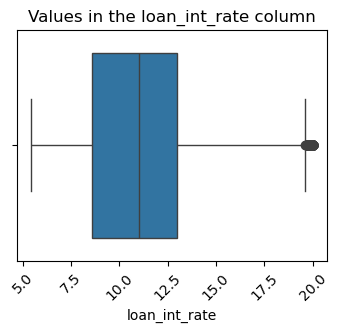
\includegraphics[width=\textwidth]{Plots/InterestRate.png}
        \caption{Interest rate}
        \label{fig:Boxplot5}
    \end{subfigure}
    \hfill
    \begin{subfigure}[b]{0.22\textwidth}
        \centering
        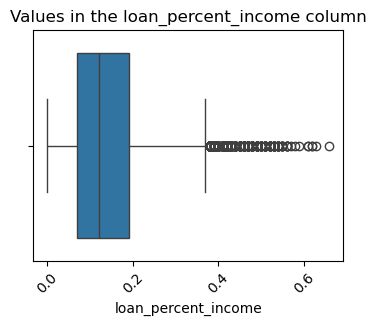
\includegraphics[width=\textwidth]{Plots/PercentIncome.png}
        \caption{Percentage of income}
        \label{fig:Boxplot6}
    \end{subfigure}
    \hfill
    \begin{subfigure}[b]{0.22\textwidth}
        \centering
        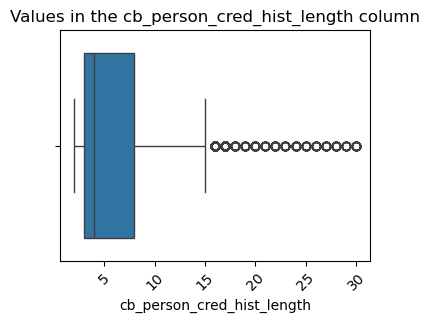
\includegraphics[width=\textwidth]{Plots/CreditHistory.png}
        \caption{Credit history length}
        \label{fig:Boxplot7}
    \end{subfigure}
    \hfill
    \begin{subfigure}[b]{0.22\textwidth}
        \centering
        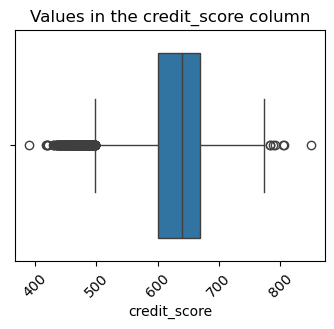
\includegraphics[width=\textwidth]{Plots/CreditScore.png}
        \caption{Credit score}
        \label{fig:Boxplot8}
    \end{subfigure}
    
    \caption{Box plots of all numerical columns.}
    \label{fig:Boxplots}
\end{figure}

\para There are many outliers in this dataset, most notably in the income column, where very few are earning millions.
Also, the age column has some outliers of extremely old people, including one aged 140, who cannot exist as the oldest 
person known was 112 before they died \autocite{sky_news_worlds_nodate}. This can therefore likely be attributed 
to erroneous generation due to this dataset being synthetic, and records with considerable outliers like this can 
be safely removed in the implementation's preprocessing phase.

\para These distributions also answer Question 1 by showing that the distribution of ages is heavily left-leaning,
with considerably more younger people getting loans than older people.

\subsubsection{Multivariate analysis}
It is also important to understand the influences that each feature has on the approval rate and other features.
Question 4 asks whether more loans are granted to men or women; it was established that there is a slight imbalance 
favouring men in the dataset in Figure \ref{fig:Bar1}, which is mirrored in Figure \ref{fig:GenderVsApproval}, which 
shows that there is no significant favouring of either gender in loan approvals when accounting for the imbalance, with a similar 
ratio of approved and rejected loans for both men and women.

\begin{figure}[H]
    \centering
    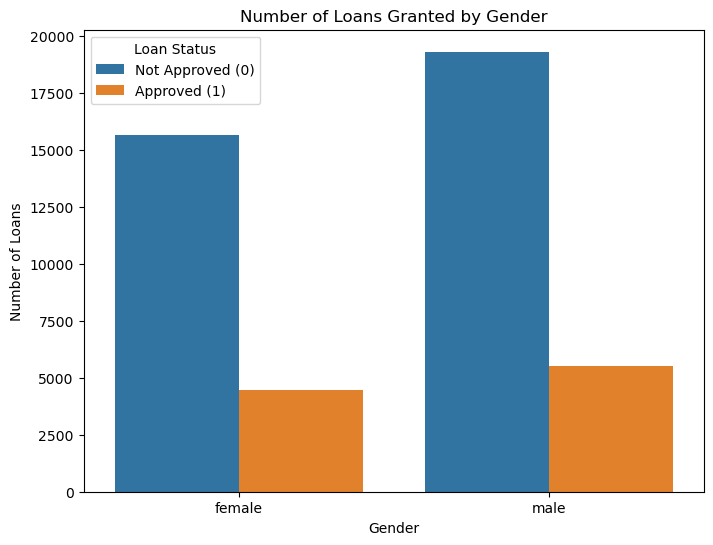
\includegraphics[width=.7\linewidth]{Plots/GenderVsApproval.png}
    \caption{The amount of loans approved for each gender. (Female: 15674 approved, 4485 denied - Male: 19326 approved, 5515 denied).}
    \label{fig:GenderVsApproval}
\end{figure}

\noindent Question 5 asks about the influence of credit score on a loan's interest rate. Figures \ref{fig:Boxplot5} and \ref{fig:Boxplot8}
show that these are both numerical columns, making them suitable for a scatter graph. 

\begin{figure}[H]
    \centering
    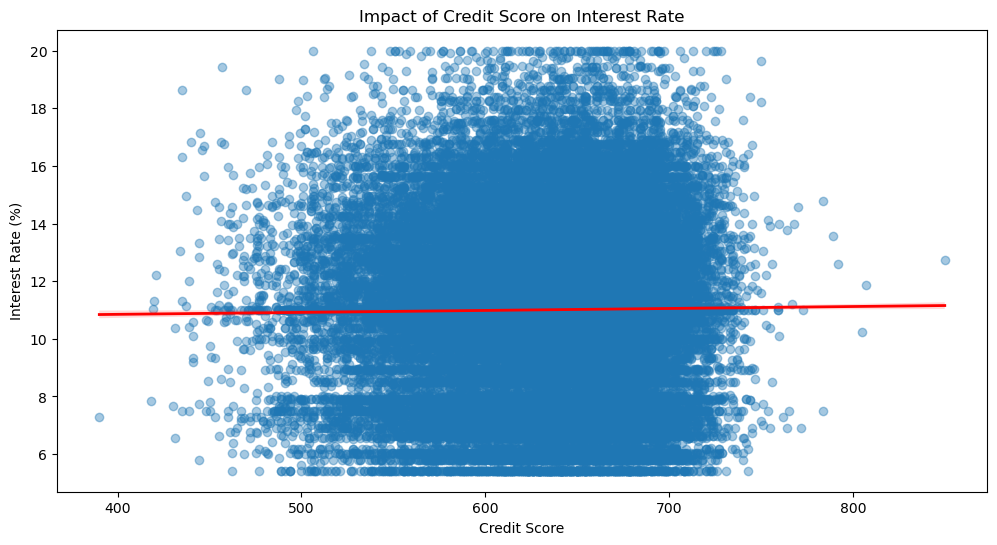
\includegraphics[width=.7\linewidth]{Plots/ScoreVsRate.png}
    \caption{A scatter plot showing the influence of credit score on interest rate.}
    \label{fig:ScoreVsRate}
\end{figure}

\para Intriguingly, Figure \ref{fig:ScoreVsRate} indicates that in this dataset there is no correlation between credit score 
and interest rate. This is unlike the real world, where higher credit scores typically correlate to lower interest rates \autocite{american_express_does_nodate},
and is likely a result of this data being synthetically generated rather than gathered from a real-world environment.


\subsubsection{Encoding}
Machine learning models cannot directly interpret string data. Therefore, strings must be encoded to numerical representations
through either label encoding or one-hot encoding. Label encoding is best suited to ordinal data as it will maintain the ordering 
of said data, such as levels of education. One-hot encoding is better suited to nominal data without an inherent order, such as 
the intent of a loan. Therefore, this dataset requires the use of both types of encoding, shown in Figures \ref{fig:LabelEncoding}
and \ref{fig:OneHotEncoding}

% REMEMBER, WHILE YOU MAY NOT NEED TO PUT IT HERE:
% DEFAULT ON LOAN SHOULD PROBABLY USE LABEL ENCODER TOO.

\begin{figure}[H]
    \centering
    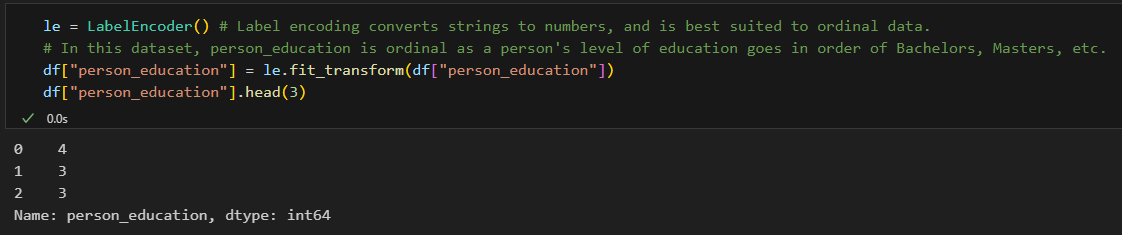
\includegraphics[width=\linewidth]{Draft Pipeline/pandas/LabelEncoding.png}
    \caption{Using label encoding for the person\_education column.}
    \label{fig:LabelEncoding}
\end{figure}

\begin{figure}[H]
    \centering
    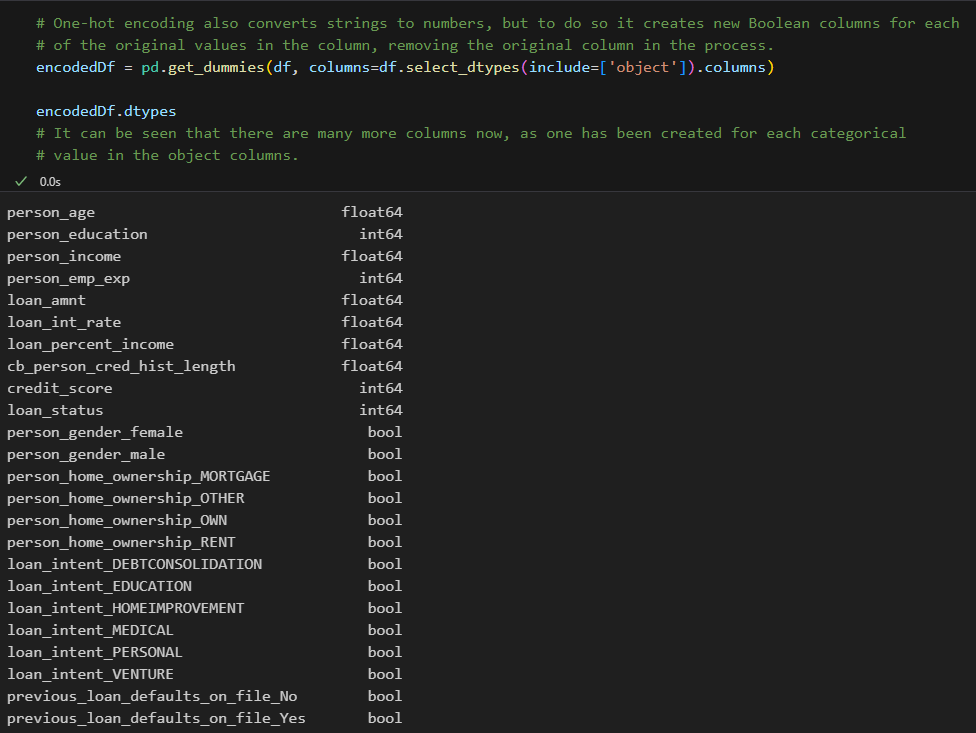
\includegraphics[width=\linewidth]{Draft Pipeline/pandas/OneHotEncoding.png}
    \caption{Using one-hot encoding for the other string columns.}
    \label{fig:OneHotEncoding}
\end{figure}

\subsubsection{Correlations}
The easiest way to view the correlations between variables is through a correlation matrix, seen below in Figure \ref{fig:BigMatrix}, which 
cannot be created unless data is first encoded. However, an immediate observation is the sheer size of the matrix due to an unfortunate side 
effect from one-hot encoding creating entirely new columns, increasing the dimensionality of the dataset. 

\begin{figure}[H]
    \centering
    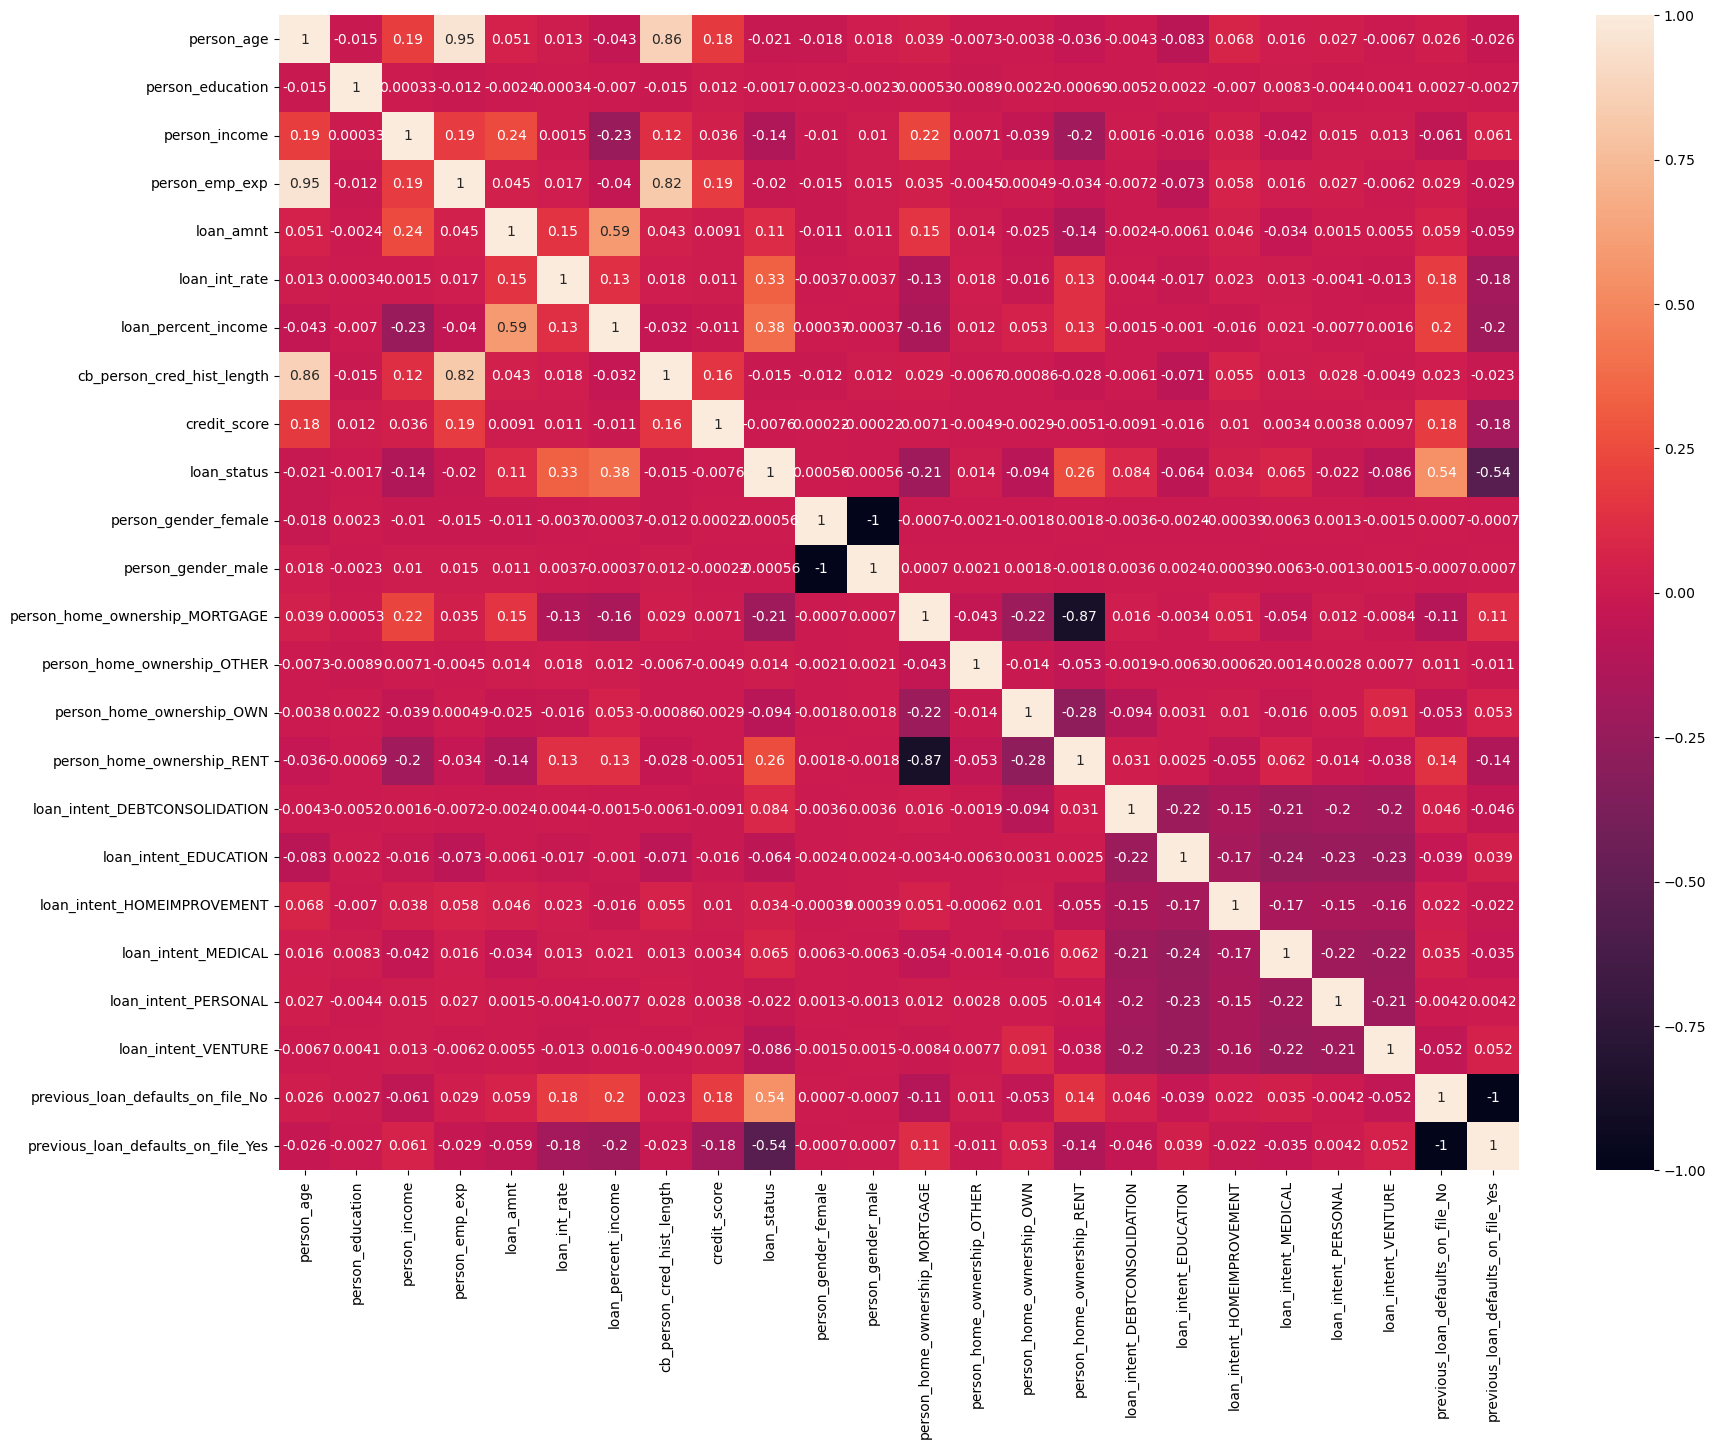
\includegraphics[width=\linewidth]{Plots/BigMatrix.png}
    \caption{The full correlation matrix for the encoded dataset.}
    \label{fig:BigMatrix}
\end{figure}

% To remedy this, the matrix can be produced after first filtering the dataset's correlations to only include rows with over 0.5 correlation 
% to each other. This is not a necessary process, but was done for easier viewing.

% \begin{figure}[H]
%     \centering
%     \includegraphics[width=\linewidth]{Plots/MiniMatrix.png}
%     \caption{The filtered correlation matrix for the encoded dataset.}
%     \label{fig:MiniMatrix}
% \end{figure}

\pagebreak 
\noindent Despite this, key insights can still be made about the likelihood of a loan being granted, such as:

\begin{itemize}
    \item Loans are most likely to be approved if the person has never defaulted on a loan before.
    \begin{itemize}
        \item They are least likely to be approved if the person has defaulted before.
    \end{itemize}
    \item The interest rate positively correlates with the loan's approval.
    \item If the person rents their home, they are more likely to be approved.
    \begin{itemize}
        \item They are less likely to be approved if they have a mortgage.
    \end{itemize}
    \item Loans are more likely to be approved if they are a large percentage of the person's yearly income.
\end{itemize}

\subsection{Research answers}
Through this extensive EDA process, the questions posed in Table \ref{tab:Questions} can now be answered:

\begin{longtable}{ | p{0.05\textwidth} | p{0.85\textwidth} | }
    \hline
    \cellcolor{blue!25} ID & \cellcolor{blue!25} Answer \\
    \hline
    1 & The age distribution of loan applicants is significantly left-leaning, with the interquartile range 
    of the feature consisting of applicants between 20 and 40 years old as shown in Figure \ref{fig:Boxplot1}. \\
    \hline
    2 & The most common loan intent is for educational purposes as revealed in Figure \ref{fig:Bar4}. While this isn't directly defined in the dataset's 
    documentation, it is a safe assumption that this refers to student loans such as those for university tuition. \\
    \hline
    3 & The correlation matrix in Figure \ref{fig:BigMatrix} states that there is an extremely slight negative correlation 
    between a loan's approval and the age of the applicant. However, given the imbalance of the dataset's ages, it can instead 
    safely be said that there is no significant correlation between applicant age and loan approval. \\
    \hline 
    4 & The dataset is imbalanced in favour of men, so there are technically more loans granted to men. However, 
    the comparison in Figure \ref{fig:GenderVsApproval} indicates that the proportions of granted to denied loans 
    is similar across both genders. This is also matched by the correlation matrix in Figure \ref{fig:BigMatrix}, 
    which showed a negligible correlation between gender and loan status. \\
    \hline 
    5 & Credit score does not affect the interest rates of loans in this dataset as shown in Figure \ref{fig:ScoreVsRate}. 
    This is unlike the real world where applicants with high credit scores can typically have lower interest rates \autocite{american_express_does_nodate}. 
    \\
    \hline 
    6 & The primary finding from the correlation matrix in Figure \ref{fig:BigMatrix} is that the strongest influential factor on 
    loan approval is whether a person has previously defaulted on a loan. If they have, they are enormously more likely to
    be rejected, whereas if they have not, they are more likely to get a loan. \\
    \hline
    \caption{The answers to Table \ref{tab:Questions}'s research questions.}\label{tab:Answers}
\end{longtable}

\section{Model Development}\label{sec:Development}
\subsection{Description}
The model development stage accepts the processed dataset from the preprocessing stage as input and leverages 
machine learning algorithms to solve the problem in question, either a classification problem where 
data will be identified as being of a certain category (class), or a regression problem where unknown 
data can be predicted. Both of these problems require the model to be "fitted" and "trained".
These refer to the utilisation of the processed dataset for the recognition of patterns, 
associations and correlations within the data. To fit and train the data, it is split into two sets:
a training set, consisting of a large majority of the data (\~80\%), and a testing set which uses the 
remaining minority. The algorithm will then use what it has learned from the training set to make predictions 
on the testing set, from which the accuracy of the model can be ascertained. These processes often yield better
results with larger datasets, as the algorithm will have more information to learn and make predictions based on,
which is why it is preferred to not remove data from the dataset unless strictly necessary.

\para This stage is conducted by machine learning engineers, and its output is that of the trained machine learning 
model, which can then be deployed and evaluated.

\subsection{In this project}
The dataset will first be loaded and deserialized via Direct-Redis. The dataset poses a classification 
problem, and as such, the Scikit-Learn Python library 
will be particularly key in this stage for its implementation of a Random Forest algorithm, which is 
reputed as one of the most accurate models in many scenarios. However, it can have a steep processing
time depending on how many decision trees it is told to create. 

\begin{longtable}{ |p{0.2\textwidth}| p{0.5\textwidth}|}
    \hline
    \cellcolor{blue!25}Software/Library & \cellcolor{blue!25}Usage for development\\
    \hline
    Direct-Redis &
    Will retrieve the dataframe from Redis and deserialize it.\\
    \hline
    % Arrow & 
    % Will deserialize the stored dataframe from Redis after the preprocessing stage.\\
    % \hline
    Pandas & 
    Will store the dataframe deserialized by Arrow.\\
    \hline
    Redis &
    Stores the processed dataset to be retrieved at the beginning of this stage.\\
    \hline
    Scikit-learn & 
    Will be used for its implementations of various algorithms, most notably a Random Forest Classifier.
    Will also provide useful metrics such as accuracy on the training and test data.\\
    \hline
    MLFlow &
    Will be used to store and track each iteration of the model that is produced as this phase is 
    repeated.\\
    \hline
\caption{Descriptions of software to be used for model development.}\label{tab:DevelopmentSoftware}
\end{longtable}

\section{Model Deployment}\label{sec:Deployment}
\subsection{Description}
The developed model from the previous stage of the pipeline can then be integrated into an actual environment,
and can be utilised as a tool to make decisions. This stage is where software engineers will make the model 
available for use, and where the model will therefore begin to be provided with unseen data, which refers to data 
outside of the original training dataset. Models are typically deployed using Representational State Transfer APIs, 
better known as REST APIs \autocite{redhat_what_nodate}. REST APIs make use of typical frontend web 
HTTP requests (GET, POST, PUT, DELETE) from the client to give instructions to the backend machine learning
model \autocite{restfulapi_what_2023}. A significant benefit of using REST APIs is the 
massive portability benefits provided; using a REST API means that the model can provide results to a 
wide variety of devices such as Windows PCs, Macs, and even phones, as anything that can make HTTP requests 
can interface with one.


\subsection{In this project}
The produced model will be hosted on a webserver via Uvicorn, and the REST API will be implemented 
via FastAPI. These two Python packages will provide an interface where the user can input the predictor 
variables of the dataset (age, credit score, etc.) to receive the model's output result.


\begin{longtable}{ |p{0.2\textwidth}| p{0.5\textwidth}|}
    \hline
    \cellcolor{blue!25}Software/Library & \cellcolor{blue!25}Usage for deployment\\
    \hline
    FastAPI &
    Will be used to provide the API between the user and the ML model, where the user will 
    give data to API endpoints and the model will supply a prediction.\\
    \hline
    Uvicorn &
    Will be used to host the webserver that the API will run on.\\
    \hline
    MLFlow &
    Will be used as a "bridge" of sorts between the user and the model, and will access and load 
    it as well as retrieving any necessary artifacts to process the data that the user supplies.\\
    \hline
\caption{Descriptions of software to be used for model deployment.}\label{tab:DeploymentSoftware}
\end{longtable}

\pagebreak

\section{Model Monitoring}\label{sec:Monitoring}
\subsection{Description}
After the model is deployed, its performance is continuously monitored by data scientists. This consists of the analysis
of the model's results via metrics such as those found in Table \ref{tab:metrics}. By monitoring the model, any issues 
with it can be quickly identified, and the pipeline can be restarted to yield a better model, which can be monitored again.  

\begin{longtable}{ |p{0.2\textwidth}| p{0.45\textwidth}| p{0.15\textwidth}|}
    \hline
    \cellcolor{blue!25}Metric & \cellcolor{blue!25}What is it? & \cellcolor{blue!25}Type\\
    \hline
    Accuracy & The number of correct predictions divided by the total amount of predictions. & Classification\\
    \hline
    Precision & The ratio of correctly predicted positives to the total amount of positives in the dataset. 
    & Classification \\
    \hline
    F1-score & A measurement calculated from a model's accuracy and precision.\autocite{kundu_f1_nodate} & Classification\\
    \hline
    Mean Absolute Error (MAE) & The average of the differences between predicted and actual values. & Regression\\
    \hline
    $R^2$ (R-Squared) & Also known as the coefficient of determination, shows how well the predicted data fits the 
    actual data \autocite{cfi_r-squared_nodate}. & Regression \\
    \hline
\caption{Descriptions of various metrics to grade ML models.}\label{tab:metrics}
\end{longtable}


\subsection{In this project}
This pipeline aims to produce a binary classification model, so getting the model's Accuracy, Precision, and F1-score will 
be useful in the evaluation of each iteration of the model. To do so, MLFlow will be used to store each iteration's 
parameters and performance metrics. 

\begin{figure}[H]
    \centering
    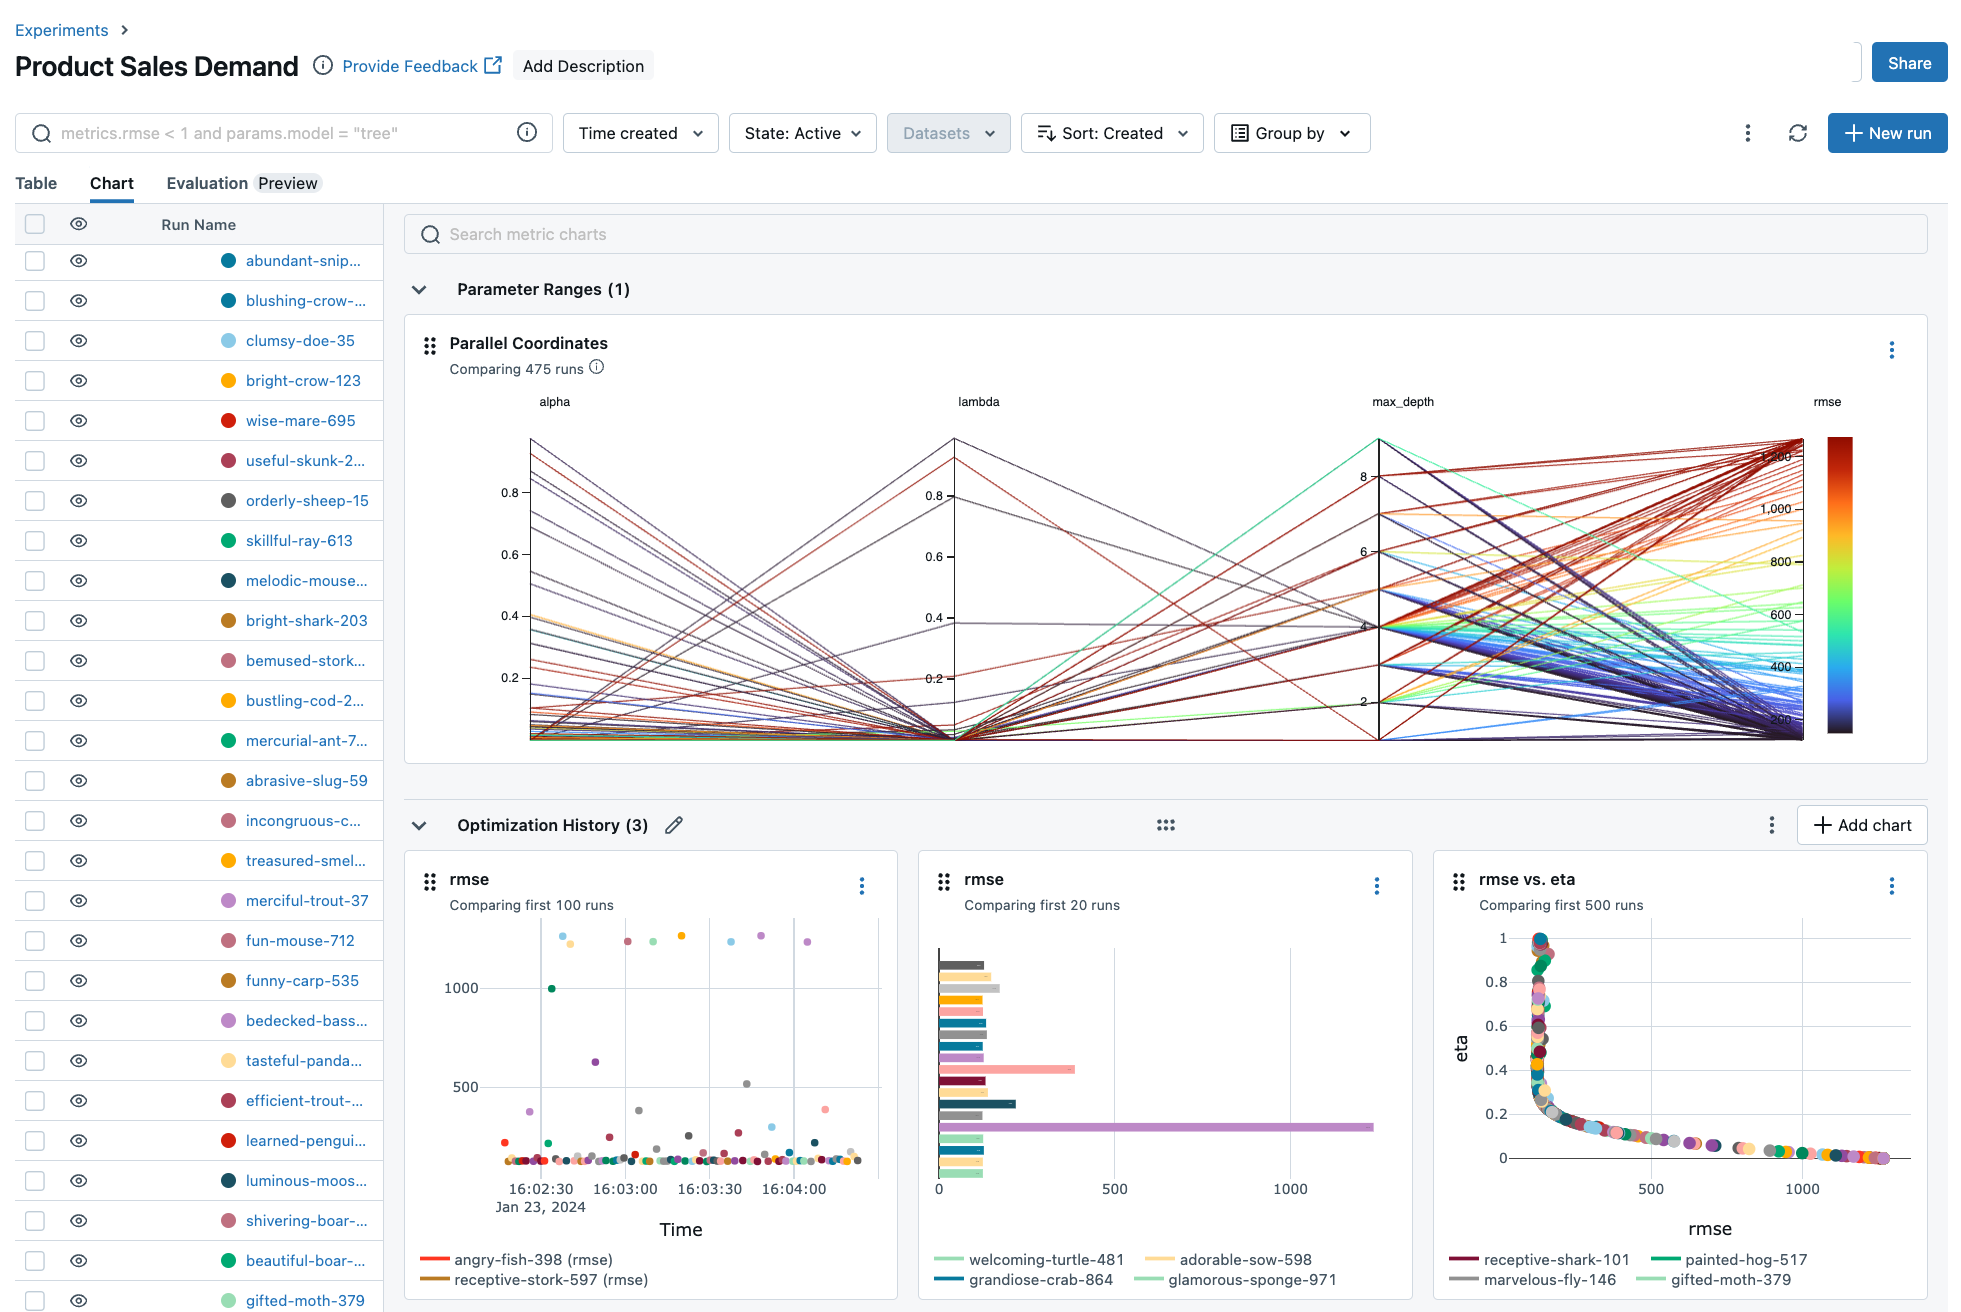
\includegraphics[width=.5\linewidth]{Draft Pipeline/MLFlowSample.png}
    \caption{An example of the MLFlow monitoring dashboard \autocite{mlflow_mlflow_nodate}.}
    \label{fig:MLFlowSample}
\end{figure}
